%!TeX encoding = UTF-8
%!TeX program = xelatex
\documentclass[notheorems, aspectratio=54]{beamer}
% aspectratio: 1610, 149, 54, 43(default), 32
\usepackage{pgfplots}

\usepackage{latexsym}
\usepackage{amsmath,amssymb}
\usepackage{mathtools}
\usepackage{color,xcolor}
\usepackage{graphicx}
\usepackage{algorithm}
\usepackage{amsthm}
\usepackage{lmodern} % 解决 font warning
% \usepackage[UTF8]{ctex}
\usepackage{animate} % insert gif

\usepackage{lipsum} % To generate test text 
\usepackage{ulem} % 下划线,波浪线

\usepackage{listings} % display code on slides; don't forget [fragile] option after \begin{frame}

\usepackage{tkz-euclide}

% arrow and line for 'tkzPointShowCoord'
\makeatletter
\tikzset{arrow coord style/.style={%
    densely dashed,
    \tkz@euc@linecolor,
    %>=stealth',
    %->,
    }}
    \tikzset{xcoord style/.style={%
    \tkz@euc@labelcolor,
    font=\normalsize,text height=1ex,
    inner sep = 0pt,
    outer sep = 0pt,
    fill=\tkz@fillcolor,
    below=6pt
    }} 
\tikzset{ycoord style/.style={%
    \tkz@euc@labelcolor,
    font=\normalsize,text height=1ex, 
    inner sep = 0pt,
    outer sep = 0pt, 
    fill=\tkz@fillcolor,
    left=6pt
    }}  
\makeatother
% ----------------------------------------------
% tikx
\usepackage{framed}
\usepackage{tikz}
\usepackage{pgf}
\usetikzlibrary{automata, calc,trees,positioning,arrows,chains,shapes.geometric,%
    decorations.pathreplacing,decorations.pathmorphing,shapes,%
    matrix,shapes.symbols}
\pgfmathsetseed{1} % To have predictable results
% Define a background layer, in which the parchment shape is drawn
\pgfdeclarelayer{background}
\pgfsetlayers{background,main}

% define styles for the normal border and the torn border
\tikzset{
  normal border/.style={orange!30!black!10, decorate, 
     decoration={random steps, segment length=2.5cm, amplitude=.7mm}},
  torn border/.style={orange!30!black!5, decorate, 
     decoration={random steps, segment length=.5cm, amplitude=1.7mm}}}

% Macro to draw the shape behind the text, when it fits completly in the
% page
\def\parchmentframe#1{
\tikz{
  \node[inner sep=2em] (A) {#1};  % Draw the text of the node
  \begin{pgfonlayer}{background}  % Draw the shape behind
  \fill[normal border] 
        (A.south east) -- (A.south west) -- 
        (A.north west) -- (A.north east) -- cycle;
  \end{pgfonlayer}}}

% Macro to draw the shape, when the text will continue in next page
\def\parchmentframetop#1{
\tikz{
  \node[inner sep=2em] (A) {#1};    % Draw the text of the node
  \begin{pgfonlayer}{background}    
  \fill[normal border]              % Draw the ``complete shape'' behind
        (A.south east) -- (A.south west) -- 
        (A.north west) -- (A.north east) -- cycle;
  \fill[torn border]                % Add the torn lower border
        ($(A.south east)-(0,.2)$) -- ($(A.south west)-(0,.2)$) -- 
        ($(A.south west)+(0,.2)$) -- ($(A.south east)+(0,.2)$) -- cycle;
  \end{pgfonlayer}}}

% Macro to draw the shape, when the text continues from previous page
\def\parchmentframebottom#1{
\tikz{
  \node[inner sep=2em] (A) {#1};   % Draw the text of the node
  \begin{pgfonlayer}{background}   
  \fill[normal border]             % Draw the ``complete shape'' behind
        (A.south east) -- (A.south west) -- 
        (A.north west) -- (A.north east) -- cycle;
  \fill[torn border]               % Add the torn upper border
        ($(A.north east)-(0,.2)$) -- ($(A.north west)-(0,.2)$) -- 
        ($(A.north west)+(0,.2)$) -- ($(A.north east)+(0,.2)$) -- cycle;
  \end{pgfonlayer}}}

% Macro to draw the shape, when both the text continues from previous page
% and it will continue in next page
\def\parchmentframemiddle#1{
\tikz{
  \node[inner sep=2em] (A) {#1};   % Draw the text of the node
  \begin{pgfonlayer}{background}   
  \fill[normal border]             % Draw the ``complete shape'' behind
        (A.south east) -- (A.south west) -- 
        (A.north west) -- (A.north east) -- cycle;
  \fill[torn border]               % Add the torn lower border
        ($(A.south east)-(0,.2)$) -- ($(A.south west)-(0,.2)$) -- 
        ($(A.south west)+(0,.2)$) -- ($(A.south east)+(0,.2)$) -- cycle;
  \fill[torn border]               % Add the torn upper border
        ($(A.north east)-(0,.2)$) -- ($(A.north west)-(0,.2)$) -- 
        ($(A.north west)+(0,.2)$) -- ($(A.north east)+(0,.2)$) -- cycle;
  \end{pgfonlayer}}}
% Define the environment which puts the frame
% In this case, the environment also accepts an argument with an optional
% title (which defaults to ``Example'', which is typeset in a box overlaid
% on the top border
\newenvironment{parchment}[1][Example]{%
  \def\FrameCommand{\parchmentframe}%
  \def\FirstFrameCommand{\parchmentframetop}%
  \def\LastFrameCommand{\parchmentframebottom}%
  \def\MidFrameCommand{\parchmentframemiddle}%
  \vskip\baselineskip
  \MakeFramed {\FrameRestore}
  \noindent\tikz\node[inner sep=1ex, draw=black!20,fill=white, 
          anchor=west, overlay] at (0em, 2em) {\sffamily#1};\par}%
{\endMakeFramed}

% ----------------------------------------------

\mode<presentation>{
    \usetheme{CambridgeUS}
    % Boadilla CambridgeUS
    % default Antibes Berlin Copenhagen
    % Madrid Montpelier Ilmenau Malmoe
    % Berkeley Singapore Warsaw
    \usecolortheme{beaver}
    % beetle, beaver, orchid, whale, dolphin
    \useoutertheme{infolines}
    % infolines miniframes shadow sidebar smoothbars smoothtree split tree
    \useinnertheme{circles}
    % circles, rectanges, rounded, inmargin
}
% 设置 block 颜色
\setbeamercolor{block title}{bg=red!30,fg=white}

\newcommand{\reditem}[1]{\setbeamercolor{item}{fg=red}\item #1}

% 缩放公式大小
\newcommand*{\Scale}[2][4]{\scalebox{#1}{\ensuremath{#2}}}

% 解决 font warning
\renewcommand\textbullet{\ensuremath{\bullet}}

% ---------------------------------------------------------------------
% flow chart
\tikzset{
    >=stealth',
    punktchain/.style={
        rectangle, 
        rounded corners, 
        % fill=black!10,
        draw=white, very thick,
        text width=6em,
        minimum height=2em, 
        text centered, 
        on chain
    },
    largepunktchain/.style={
        rectangle,
        rounded corners,
        draw=white, very thick,
        text width=10em,
        minimum height=2em,
        on chain
    },
    line/.style={draw, thick, <-},
    element/.style={
        tape,
        top color=white,
        bottom color=blue!50!black!60!,
        minimum width=6em,
        draw=blue!40!black!90, very thick,
        text width=6em, 
        minimum height=2em, 
        text centered, 
        on chain
    },
    every join/.style={->, thick,shorten >=1pt},
    decoration={brace},
    tuborg/.style={decorate},
    tubnode/.style={midway, right=2pt},
    font={\fontsize{10pt}{12}\selectfont},
}
% ---------------------------------------------------------------------

% code setting
\lstset{
    language=C++,
    basicstyle=\ttfamily\footnotesize,
    keywordstyle=\color{red},
    breaklines=true,
    xleftmargin=2em,
    numbers=left,
    numberstyle=\color[RGB]{222,155,81},
    frame=leftline,
    tabsize=4,
    breakatwhitespace=false,
    showspaces=false,               
    showstringspaces=false,
    showtabs=false,
    morekeywords={Str, Num, List},
}

% ----

% ---------------------------------------------------------------------

%% preamble
\title{Foundation of Analytics: Lecture 2}
% \subtitle{The subtitle}
\author{Dihui Lai}
\institute[WUSTL]{dlai@wustl.edu}

% -------------------------------------------------------------

\begin{document}

%% title frame
\begin{frame}
    \titlepage
\end{frame}

%% normal frame
\section{Introduction to Statistics: Random Variable}
\begin{frame}
CONTENT
\begin{itemize}
\item Discrete Random Variable 
\item Continuous Random Variable
\item Demo
\end{itemize}
\end{frame}


\begin{frame}
\begin{parchment}[Example 1: Roll a dice]
There six possible outcome of rolling a dice i.e. "1", "2", "3", ... "6".  
\begin{itemize}
\item If I roll a dice 60 times, how many times do you get "1"?
\item What is the probability of getting "1"? 1/6?
\end{itemize}
\end{parchment}
\end{frame}


\begin{frame}
\frametitle{Dice-Rolling: Expectation, Variance etc.}
\begin{itemize}
\item Unique values: $1, 2, 3, 4, 5, 6$
\item min:1; max:6
\item expectation: $\frac{\sum{\mathnormal{x_i}}}{\mathnormal{N}}$?
\item variance: ?

\end{itemize}

\end{frame}

\begin{frame}
\frametitle{Random Variable}

A \textbf{random variable} $\mathnormal{X}$  can take different values with certain probability. To understand a random variable, we need to consider two things: 
\begin{itemize}
\item The possible outcome value of an experiment: $\mathnormal{x}$ 
\item The probability of an outcome is $\mathnormal{x}$: $\mathnormal{P(x)}$.

\end{itemize}

\end{frame}


\begin{frame}
\frametitle{Discrete Random Variable}

A discrete random variable $\mathnormal{X}$ 
\begin{itemize}
\item Can take k possible values $\mathnormal{x_{1}}$, $\mathnormal{x_{2}}$, $\mathnormal{x_{3}}$ ... $\mathnormal{x_{k}}$
\item Each with probability of $\mathnormal{p_{1}}$, $\mathnormal{p_{2}}$, $\mathnormal{p_{3}}$ ... $\mathnormal{p_{k}}$. For simplicity, we denote the probabilities using a probability mass function $$\mathnormal{P(x_i)=p_{i}}, \mathnormal{i}=1, 2, 3, ...\mathnormal{k}$$
\item The probabilities for all possible values sum up to be $1$, i.e. $\mathnormal{\sum_{i=1}^{k}p_{i}}=1$
\end{itemize}

\end{frame}


\begin{frame}
\frametitle{Histogram/Distribution of Discrete Variables}
\begin{itemize}
\item For data of discrete values e.g. $\mathnormal{x^T=[x^{1}, x^{2}, x^{3} ..., x^{n}]}$, 
\item Find the unique value of the data
\item Count the number of data occured at each discrete value $\mathnormal{N_i}$. The total number of data points $\mathnormal{N=\sum_{i}N_i}$. The empirical probability mass function can be estimated by $$\mathnormal{P(x_i)=\frac{N_i}{N}}$$

\end{itemize}
\end{frame}


\begin{frame}
\frametitle{Dice-Rolling: Distribution}
Given a series of data, $ [1, 2, 1, 3, 4, 6, 6, 4, 5, 5, ... ]$. What can you tell about the underlying story? Is it from a dice-rolling process? 

\vspace{3mm}

Count the number of occurence for each value 1, 2, 3, 4, 5, 6
%---------------------------------------------------------------%
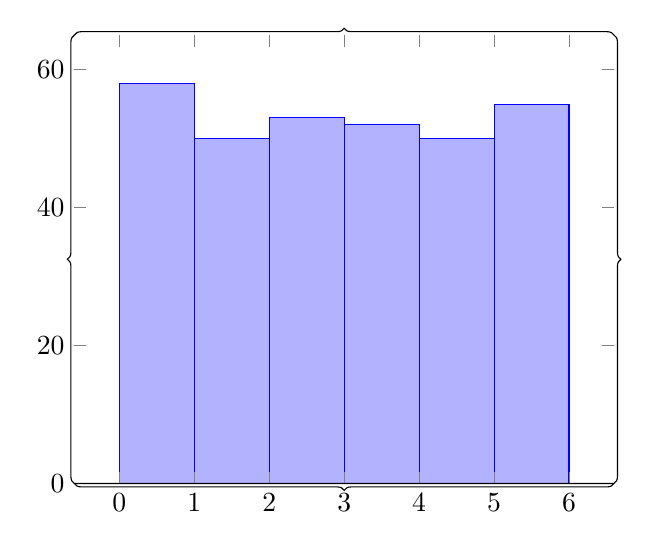
\begin{tikzpicture}
\begin{axis}[
    ymin=0, ymax=65,
    minor y tick num = 0,
    area style,
    ]
\addplot+[ybar interval,mark=no] plot coordinates { (0, 58) (1, 50) (2, 53) (3, 52) (4, 50) (5, 55) (6, 57) };
\end{axis}
\end{tikzpicture}
\end{frame}

\begin{frame}
\frametitle{Discrete Random Variable: Function and Expectation}
The expectation of a function, $\mathnormal{g(X)}$ is given by 

$$\mathnormal{E[g(X)]=\sum_{i=1}^kg(x_i)P(x_i)}$$
\end{frame}
\begin{frame}

\frametitle{Discrete Random Variable: Expectation, Variance and Moments}
In special case when $\mathnormal{g(X)=X^{n}}$, we have the $\mathnormal{n^{th}}$ raw moment of $\mathnormal{X}$

$$\mathnormal{E[X^{n}]=\sum_{i=1}^{k} x_{i}^{n} P(x_i)}$$

The expectation of $\mathnormal{X}$ is the $1^{st}$ raw moment of X 
$$\mathnormal{\mu=E[X]}$$
 
The variance of $\mathnormal{X}$ is the $\mathnormal{2^{nd}}$ moment of $\mathnormal{X}$ about the expectation  $$\mathnormal{\sigma^{2}=E[(X-\mu)^{2}]}$$
\end{frame}


\begin{frame}
\frametitle{Bernoulli Distribution}
Consider a random variable $\mathnormal{X}$ that can take value $1$ with probability $\mathnormal{p}$ and $0$ with probability $1-\mathnormal{p}$.

$$    
\mathnormal{P(x)} =
    \left\{
        \begin{array}{cc}
                \mathnormal{p} & \mathrm{if\ } \mathnormal{x}=1 \\
                1-\mathnormal{p} & \mathrm{if\ } \mathnormal{x}=0 \\
        \end{array} 
    \right.
$$
The expectation of $\mathnormal{X}$ is 
$$
\mathnormal{E[X]=p}
$$

The variance of $\mathnormal{X}$ is
$$
\mathnormal{E[(X-\mu)^2]}=\mathnormal{p}(1-\mathnormal{p})
$$
\end{frame}


\begin{frame}
\frametitle{Joint Distribution and Algerbra of Ramdom Variables}
If we create a random variable from two random variables: $$\mathnormal{Z=X+Y}$$

Distribution: $\mathnormal{f(z)}$

Expectation: $$\mathnormal{E[Z]=E[X+Y]=E[X]+E[Y]=E[Y]+E[X]}$$

Variance:
$$\mathnormal{Var[Z]}=\mathnormal{Var[X+Y]}=\mathnormal{Var[X]}+2\mathnormal{Cov[X,Y]}+\mathnormal{Var[Y]}$$

Covariance is defined as 
$$\mathnormal{{Cov}[X, Y]
={E}\left[\left(X - {E}\left[X\right]\right) \left(Y - {E}\left[Y\right]\right)\right]}$$
\end{frame}

\begin{frame}
\frametitle{Algerbra of Multiple Random Varaibles}
Expectation: $$\mathnormal{E\left(\sum_{i=1}^n X_i\right)=\sum_{i=1}^n E\left( X_i\right)}$$
Variance: $$\mathnormal{{Var}\left(\sum_{i=1}^n X_i\right)= \sum_{i=1}^n {Var}(X_i)+ \sum_{i,j}{Cov}(X_i,X_j)}$$
\end{frame}



\begin{frame}
\frametitle{Binomial Distribution}
Consider a random event whose outcome is the summation of n independent Bernoulli distribution. The distribution of the corresponding random variable $\mathnormal{X}$ can be described as

$$ \mathnormal{P(x) =  {{n}\choose{k}} p^xq^{n-x}, x=}0, 1, 2, ...\mathnormal{n}$$
The expectation of $\mathnormal{X}$ is 
$$
\mathnormal{E[X]=np}
$$

The variance of $\mathnormal{X}$ is
$$
\mathnormal{E[(X-\mu)^2]=np(}1-\mathnormal{p)}
$$
\end{frame}

\begin{frame}
\frametitle{Poisson Distribution}
Consider a random event, the probability of 1 occurence within a unit time is $p$. What's the probability distribution of events occurence within time interval of $\tau$ (e.g. No. of car accidents occurs in a day in MO). The distribution of the discrete random variable $\mathnormal{X}$ is 
$$
\mathnormal{P\left( x \right) = \frac{{e^{ - \lambda } \lambda ^x }}{{x!}}, x = 0, 1, 2, ..}
$$

The expectation of $\mathnormal{X}$ is 
$$
\mathnormal{E[X]=\lambda}
$$

$\lambda$  is the average number of events per interval, $\lambda=p\tau$

The variance of $\mathnormal{X}$ is
$$
\mathnormal{E[(X-\mu)^2]=\lambda}
$$
\end{frame}


\begin{frame}
\frametitle{Understand the Distribution of Continuous Data}
How about real value data, $[-1.407, 0.412, -1.198, 1.552, ...]$? 

\vspace{3mm}
Count the number of data points that falls into the intervals of $[-2, -1.5), [-1.5, -1.0), ... [0, 0.5), [0.5, 1) ...$

%---------------------------------------------------------------%
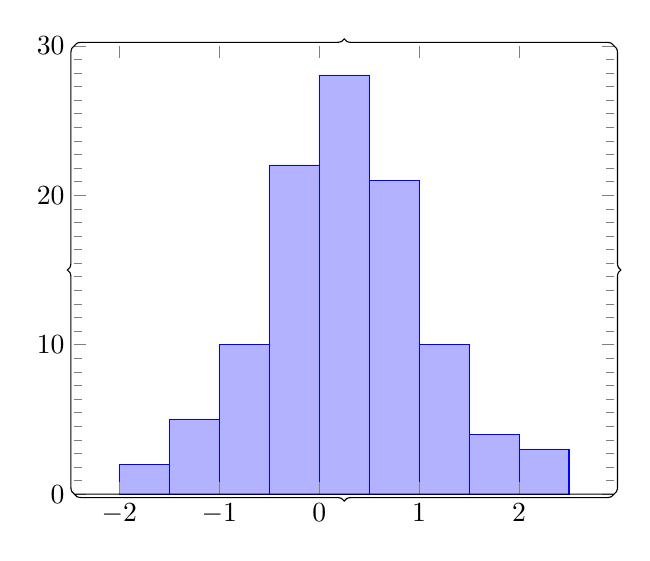
\begin{tikzpicture}
\begin{axis}[
    ymin=0, ymax=30,
    minor y tick num = 10,
    area style,
    ]
\addplot+[ybar interval,mark=no] plot coordinates { (-2, 2) (-1.5, 5) (-1, 10) (-0.5, 22) (0, 28) (0.5, 21) (1,10) (1.5, 4) (2, 3) (2.5, 1)};
\end{axis}
\end{tikzpicture}
\end{frame}


\begin{frame}
\frametitle{Histogram/Empirical Distribution of Continous Variables}
\begin{itemize}
\item For data of discrete values, count the number of data occured at each discrete value $\mathnormal{N_i}$. The total number of data points $\mathnormal{N=\sum_{i}N_i}$. The empirical probability mass function is given by $$\mathnormal{P(x_i)=\frac{N_i}{N}}$$
\item For data of continous values, define k equal-sized-bins (e.g. $\mathnormal{[x_i-\Delta x, x_i+\Delta x)}, i=1, 2, 3, ...\mathnormal{k}$). Count the number of data belong to each bin $\mathnormal{N_i}$, the total number of data points $\mathnormal{N=\sum_{i}^{k}N_i}$. The empirical probability distribution is given by $$\mathnormal{P(x_i-\Delta x \leq x < x_i+\Delta x )=\frac{N_i}{N}}$$

\end{itemize}
\end{frame}


\begin{frame}
\frametitle{Continuos Random Variable}

A continous random variable $\mathnormal{X}$
\begin{itemize}
\item Can have a range of values e.g. $\mathnormal{(-\infty, +\infty)}$, $\mathnormal{[0, 1)}$, $\mathnormal{[0, +\infty)}$
\item The probability that $\mathnormal{a\leq x \leq b}$ is defined as 

$$\mathnormal{P(a\leq x \leq b) = \int_{a}^{b} f(x) dx}$$ 

where $\mathnormal{f(x)}$ is the probability density function. Note: $\mathnormal{f(x)}$ is not probability
\item The pdf $\mathnormal{f(x)}$ has to satisfy the following propery $$\mathnormal{P(-\infty \leq x \leq +\infty) = \int_{-\infty }^{+\infty }f(x)dx=1}$$
\end{itemize}

\end{frame}

\begin{frame}
\frametitle{Continuos Random Variable: Function and Expectation}
If we denote a function of a random variable as $\mathnormal{g(X)}$, the expectation of $\mathnormal{g(X)}$ is given by
$$\mathnormal{E[g(X)]=\int_{-\infty }^{+\infty }g(x)f(x)dx}$$

\end{frame}

\begin{frame}
\frametitle{Continuos Random Variable: Expectation, Variance and Moments}
In a special case, when $\mathnormal{g(X)=X^{n}}$, the expectation of $\mathnormal{g(X)}$ is called the $\mathnormal{n^{th}}$ raw moment of $\mathnormal{X}$

$$\mathnormal{E[X^{n}]=\int_{-\infty }^{+\infty }x^{n}f(x)dx}$$

The expectation of $\mathnormal{X}$ is the $\mathnormal{1^{st}}$ raw moment of $\mathnormal{X}$ 
$$\mathnormal{\mu=E[X]}$$
 
The variance of $\mathnormal{X}$ is the $\mathnormal{2^{nd}}$ moment of $\mathnormal{X}$ about the expectation  $$\mathnormal{\sigma^{2}=E[(X-\mu)^{2}]}$$

\end{frame}


\begin{frame}
\frametitle{Calculate Expectation using Empirical Probability Distribution}

\begin{align*}
 \mathnormal{\mu} &= \mathnormal{\sum_{i=1}^k x_i f(x_i-\Delta x \leq x < x_i+\Delta x )(2\Delta x)}\\
     &=\mathnormal{\sum_{i=1}^k x_i P(x_i-\Delta x \leq x < x_i+\Delta x )}\\
     &\mathnormal{=\frac{\sum_{i=1}^k x_i N_i}{N}}
\end{align*}

\end{frame}

\begin{frame}
\frametitle{Uniform Distribution}

A uniform distribution is given by
\begin{align*}
\mathnormal{f(x)} =
    \left\{
        \begin{array}{cc}
              \mathnormal{0} & \mathrm{if\ } \mathnormal{x<a} \\
              \frac{1}{\mathnormal{b-a}}  & \mathnormal{\mathrm{if\ } a\leq x \leq b} \\
              \mathnormal{0} & \mathrm{if\ } \mathnormal{x>b} \\
        \end{array} 
    \right.
\end{align*}

\begin{center}
\begin{tikzpicture}
\tkzInit[xmax=0.8,xstep=0.2,ymax=0.65,ystep=0.2]
\tkzDrawX[noticks,label={$\mathnormal{x}$}]
\tkzDrawY[noticks,label={$\mathnormal{f(x)}$}]
\tkzDefPoint(0.2,0.6){A}
\tkzDefPoint(0.6,0.6){B}
\tkzDefShiftPoint[A](-90:3){AB}
\tkzDefShiftPoint[B](-90:3){BB}
\tkzDefShiftPoint[AB](0:-0.8){ABL}
\tkzDefShiftPoint[BB](0:0.8){BBR}
\tkzPointShowCoord[xlabel=$a$,ylabel=$\frac{1}{b-a}$](A)
\tkzPointShowCoord[xlabel=$b$](B)
\tkzDrawSegments[color=black,thick](A,B AB,ABL BB,BBR)
\tkzDrawPoints[color=black,fill=black,size=6pt](A,B)
\tkzDrawPoints[color=black,fill=white,size=6pt](AB,BB)
\end{tikzpicture}
\end{center}
\end{frame}

\begin{frame}
\frametitle{Gaussian Distribution}
A continuous random variable $Z$ is called a standard normal if
$$\mathnormal{f(Z) = \frac{1}{\sqrt{2\pi}}e^{-z^2/2}}$$
The probability of $\mathnormal{z\leq z_0}$ is given by
$$\mathnormal{P(Z\leq z_0)} = \mathnormal{\int_{-\infty}^{z_{0}}}
\frac{1}{\mathnormal{\sqrt{2}}e^{-\mathnormal{z}^2/2}}\mathnormal{dz}$$ Let $\mathnormal{X=\mu+\sigma Z}$. Then $\mathnormal{X}$
is a normal distribution with parameters $\mathnormal{\mu}$ and $\mathnormal{\sigma^2}$. Its
density function is given by
$$\mathnormal{f(x)} = \frac{1}{\mathnormal{\sqrt{2\pi}\sigma}}\mathnormal{e^{-(x-\mu)^2/2\sigma^2}}.$$ 

The expectation of $\mathnormal{X}$: $\mathnormal{E[X]=\mu}$

The variance of $\mathnormal{X}$: $\mathnormal{E[(X-\mu)^2]=\sigma^2}$
\end{frame}

\begin{frame}
\frametitle{}
\begin{center}
 Demo in Python
\end{center}
\end{frame}


\end{document}
